\documentclass[../../main.tex]{subfiles}

\begin{document}

\subsection{Overview}

Immediately after the implementation of a component, it should be unit tested; if needed, a driver can be used in place of the components that are not yet fully implemented. 
As a consequence of choosing a bottom-up approach in the implementation process, we should choose a bottom-up strategy also for integration and testing as well. 
After the unit tests of a component succeeds, it is integrated in the system and integration testing is performed: every interface that the component uses is tested. Since a bottom-up approach is used, this process ends when the components at the top of the hierarchy are integrated in the system.
At that point, the system as a whole can be tested with system tests.

\subsection{Plan}

\begin{enumerate}

	\noindent\begin{minipage}{0.9\textwidth}

	\item At first, the DBMS API has to be tested, in order to check for misconfiguration and correctness of the interface.

	\begin{figure}[H]
    \centering
    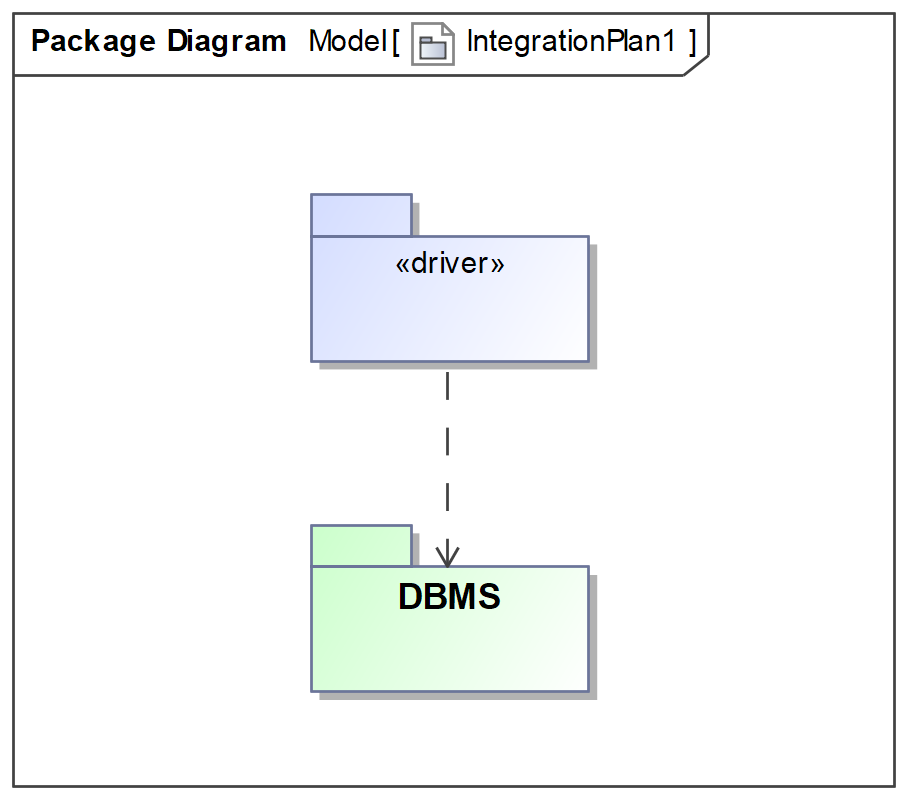
\includegraphics[width=8cm]{package__IntegrationPlan1.png}
	\end{figure}

	\end{minipage}

	\noindent\begin{minipage}{0.9\textwidth}
		
	\item Then, the implementation goes on for StoreManager, ReceiptManager, StatisticComputationManager, and LineUpSuggestionsManager. 
	
	\begin{figure}[H]
    \centering
    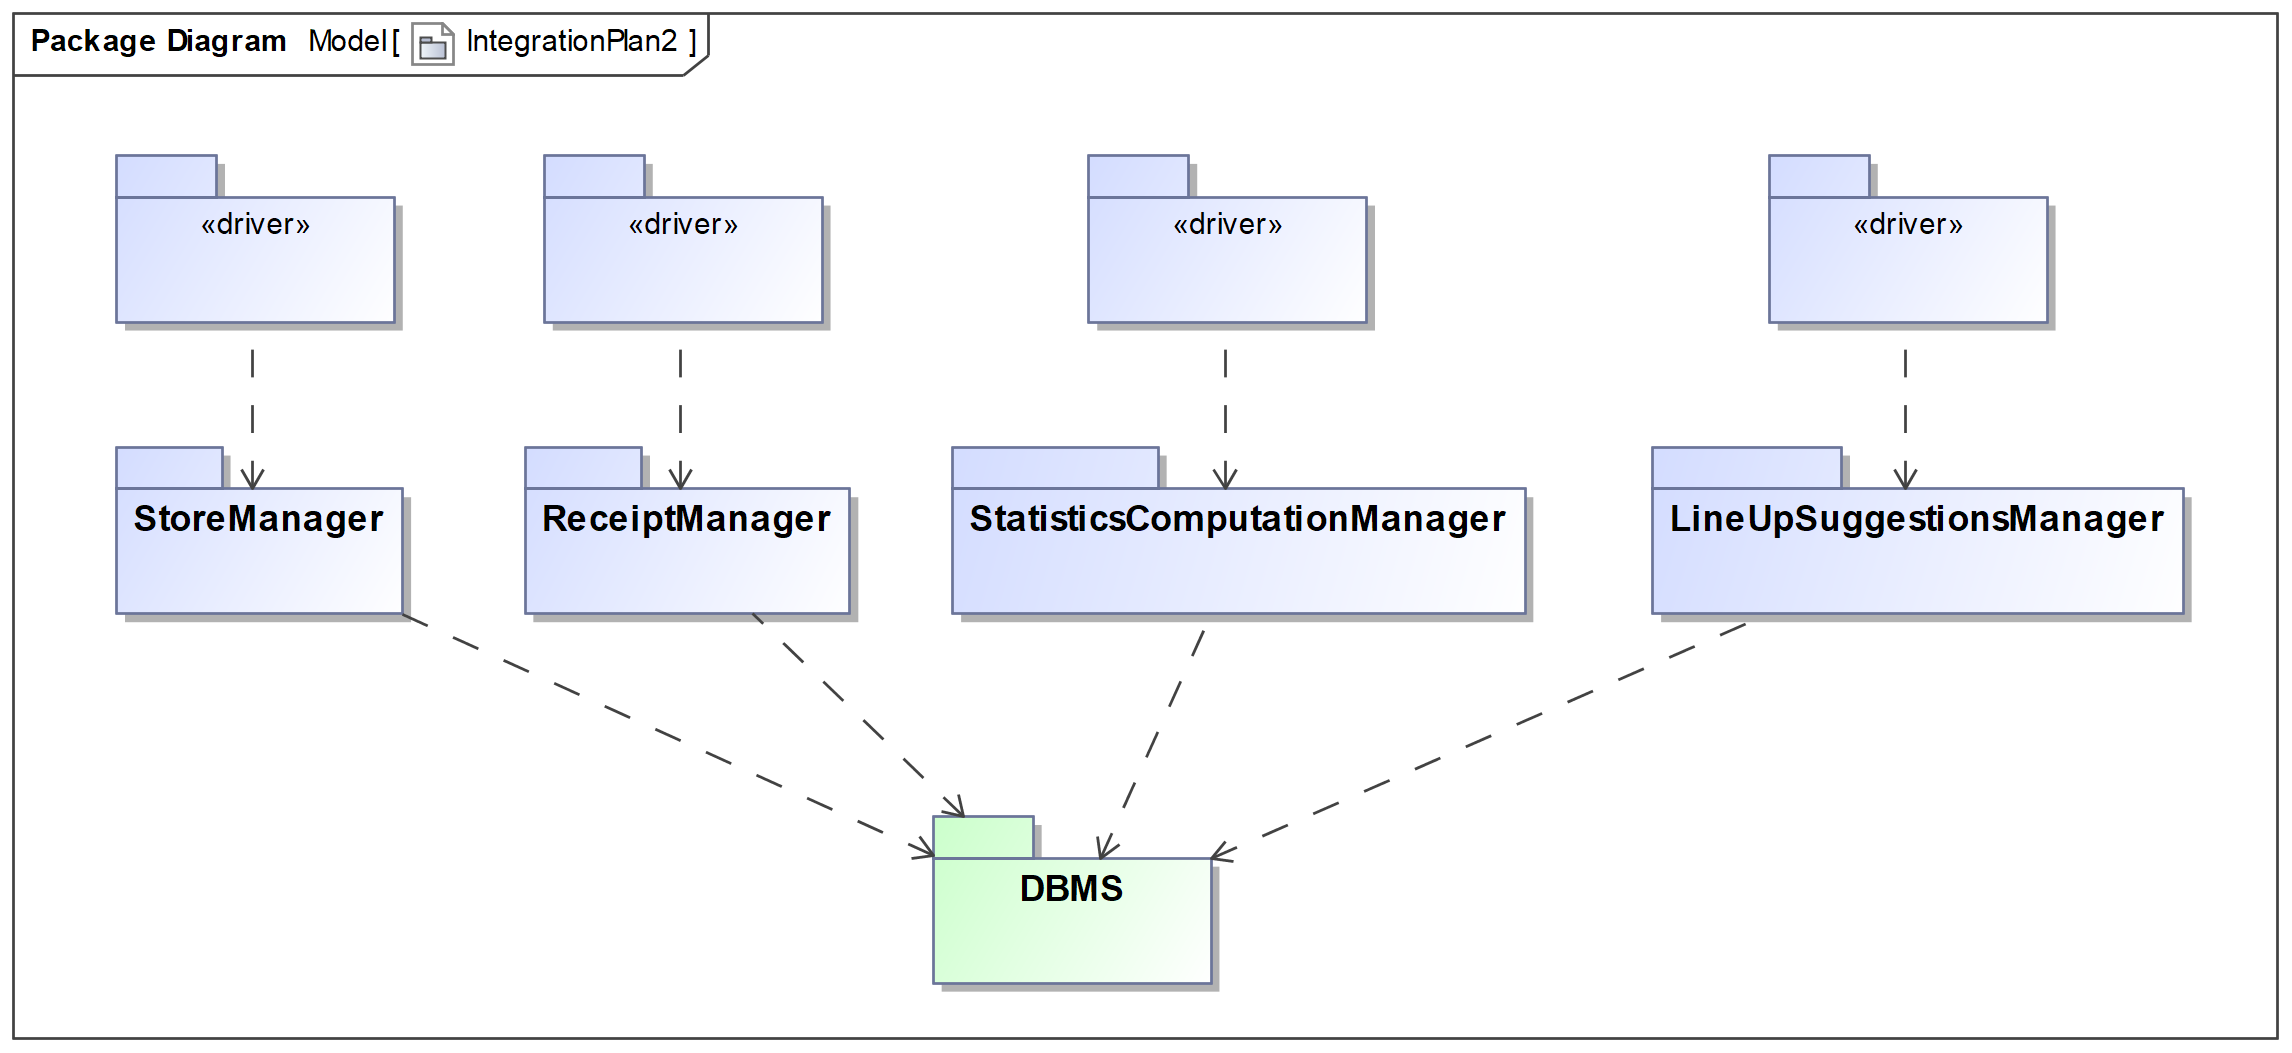
\includegraphics[width=15cm]{package__IntegrationPlan2.png}
	\end{figure}

	\end{minipage}

	\noindent\begin{minipage}{0.9\textwidth}
	
	\item Then, AccessManager, LineUpCancellationManager, and LineUpRequestManager are integrated and tested.
	
	\begin{figure}[H]
    \centering
    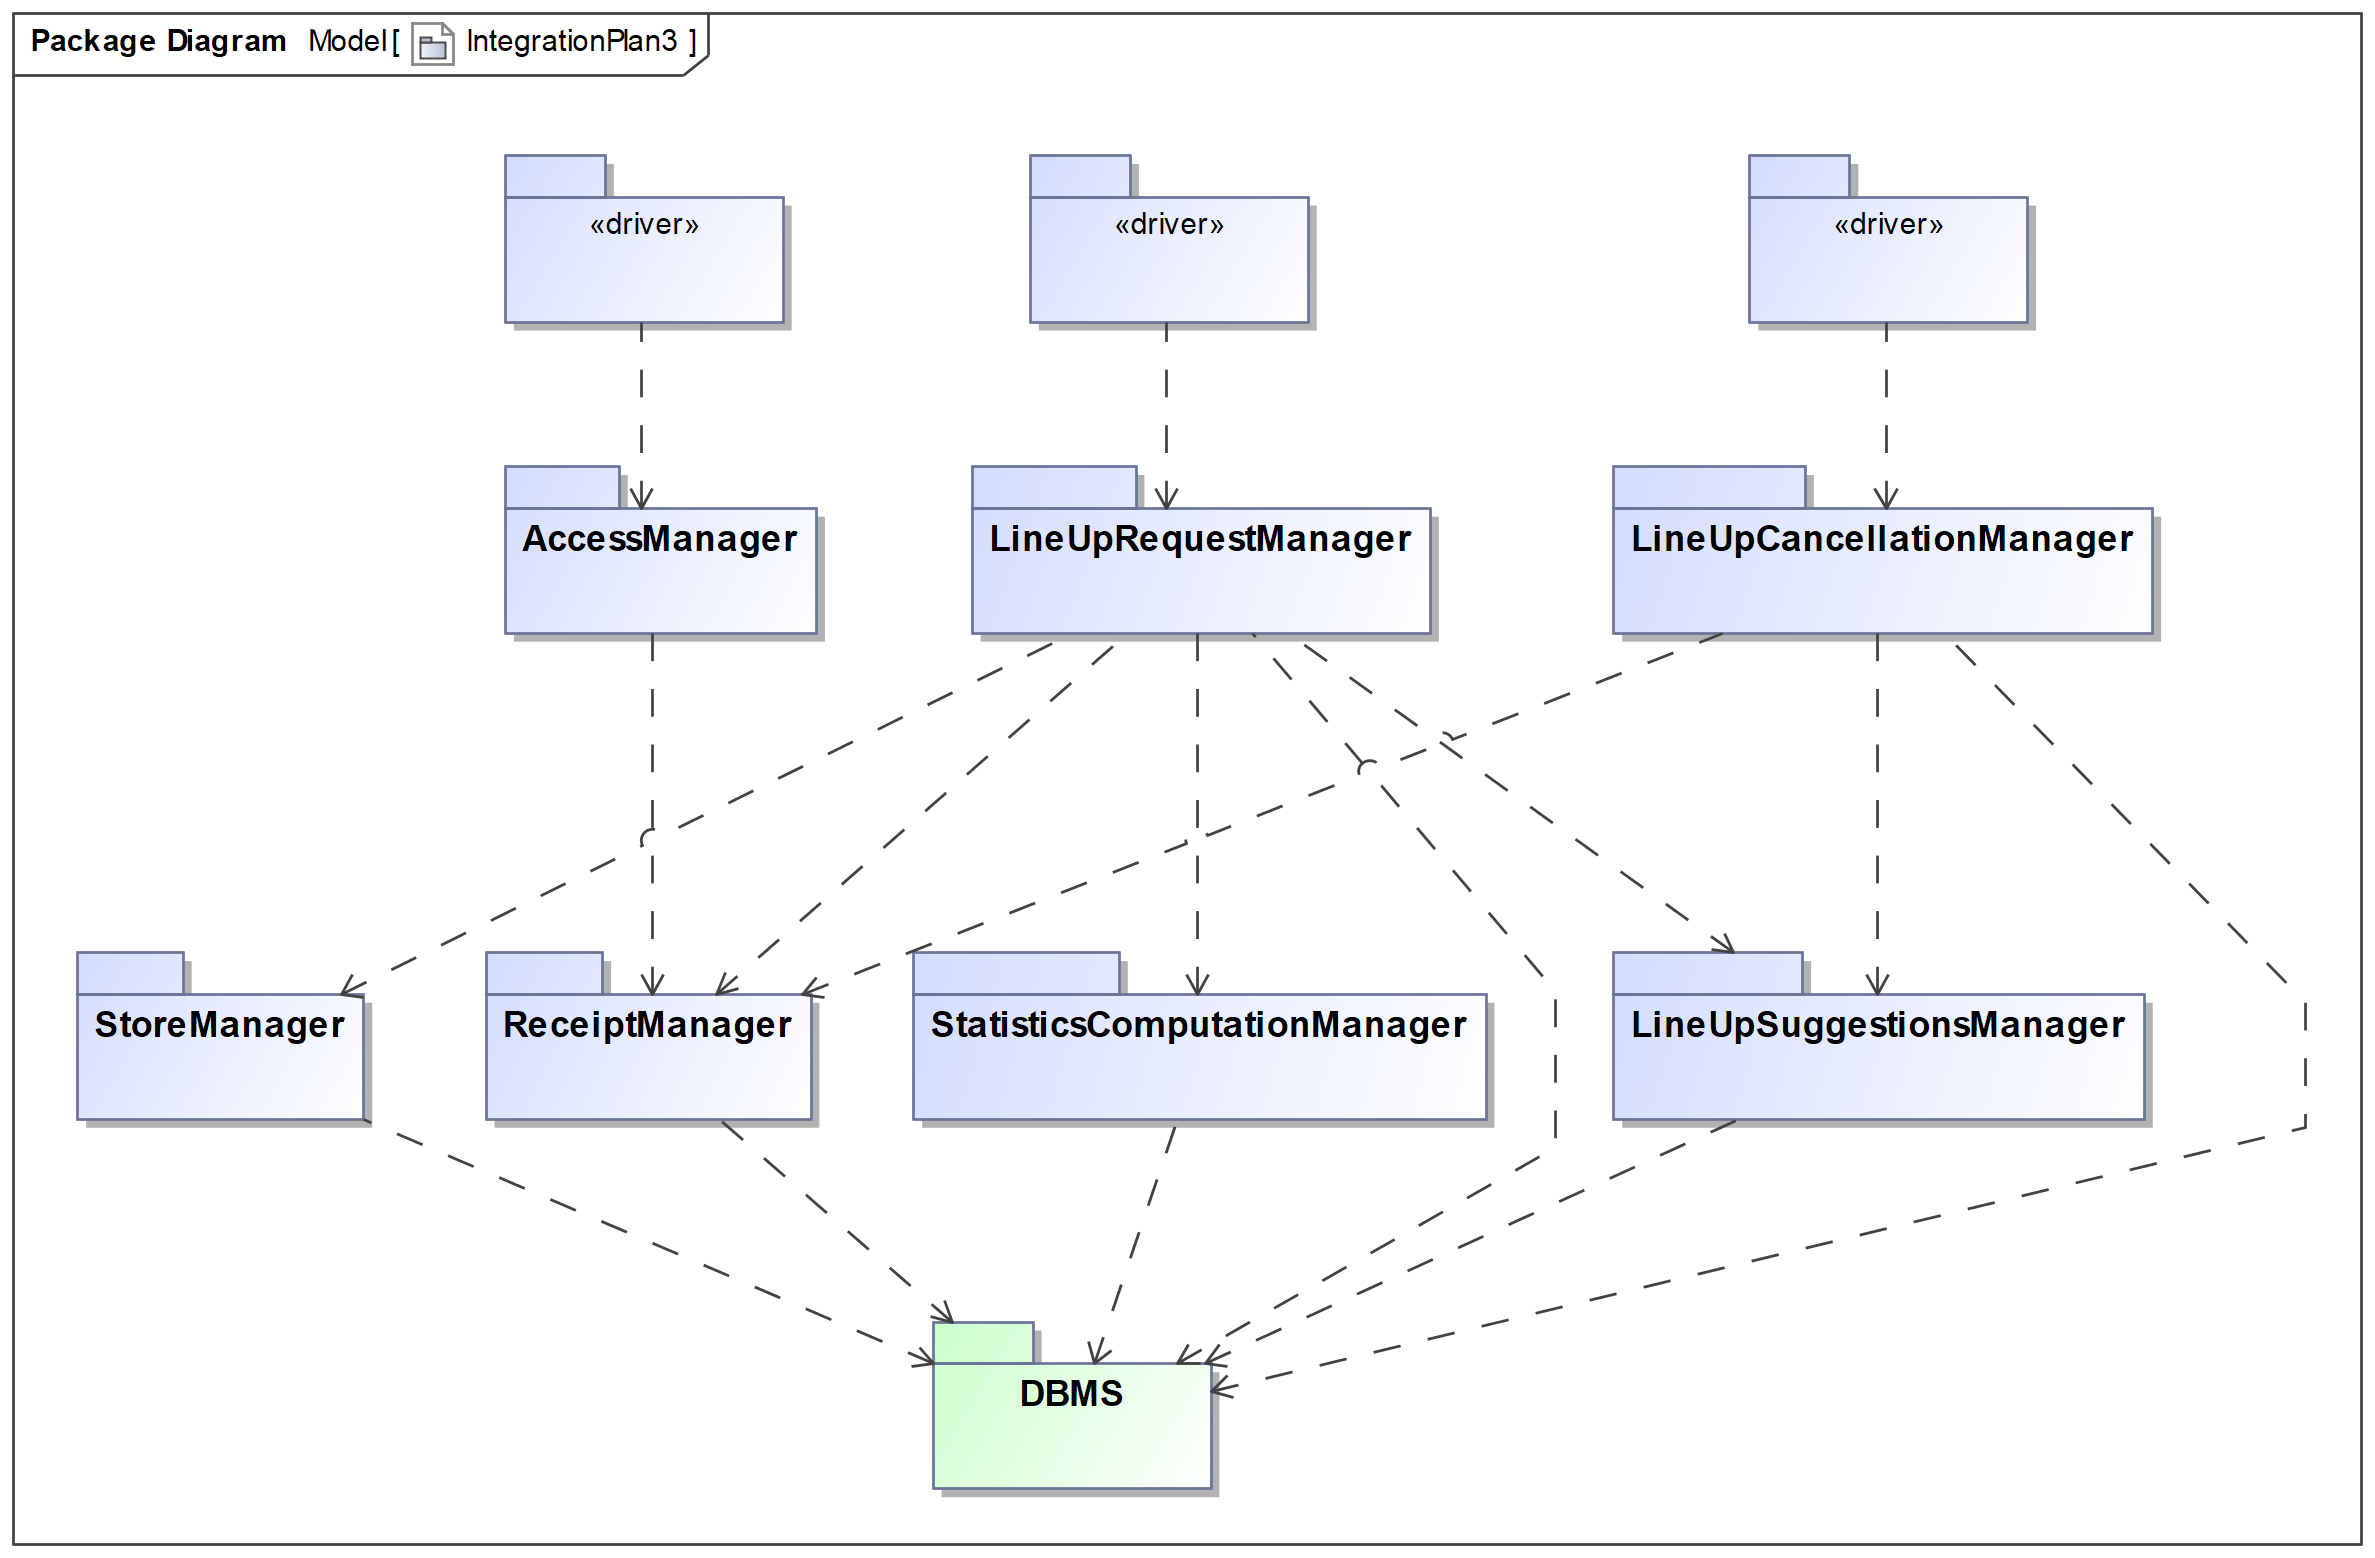
\includegraphics[width=15cm]{package__IntegrationPlan3.png}
	\end{figure}

	\end{minipage}

	\noindent\begin{minipage}{0.9\textwidth}
	
	\item Later, the implementation of NotificationManager and its integration with Notification Service can begin. 

	\begin{figure}[H]
    \centering
    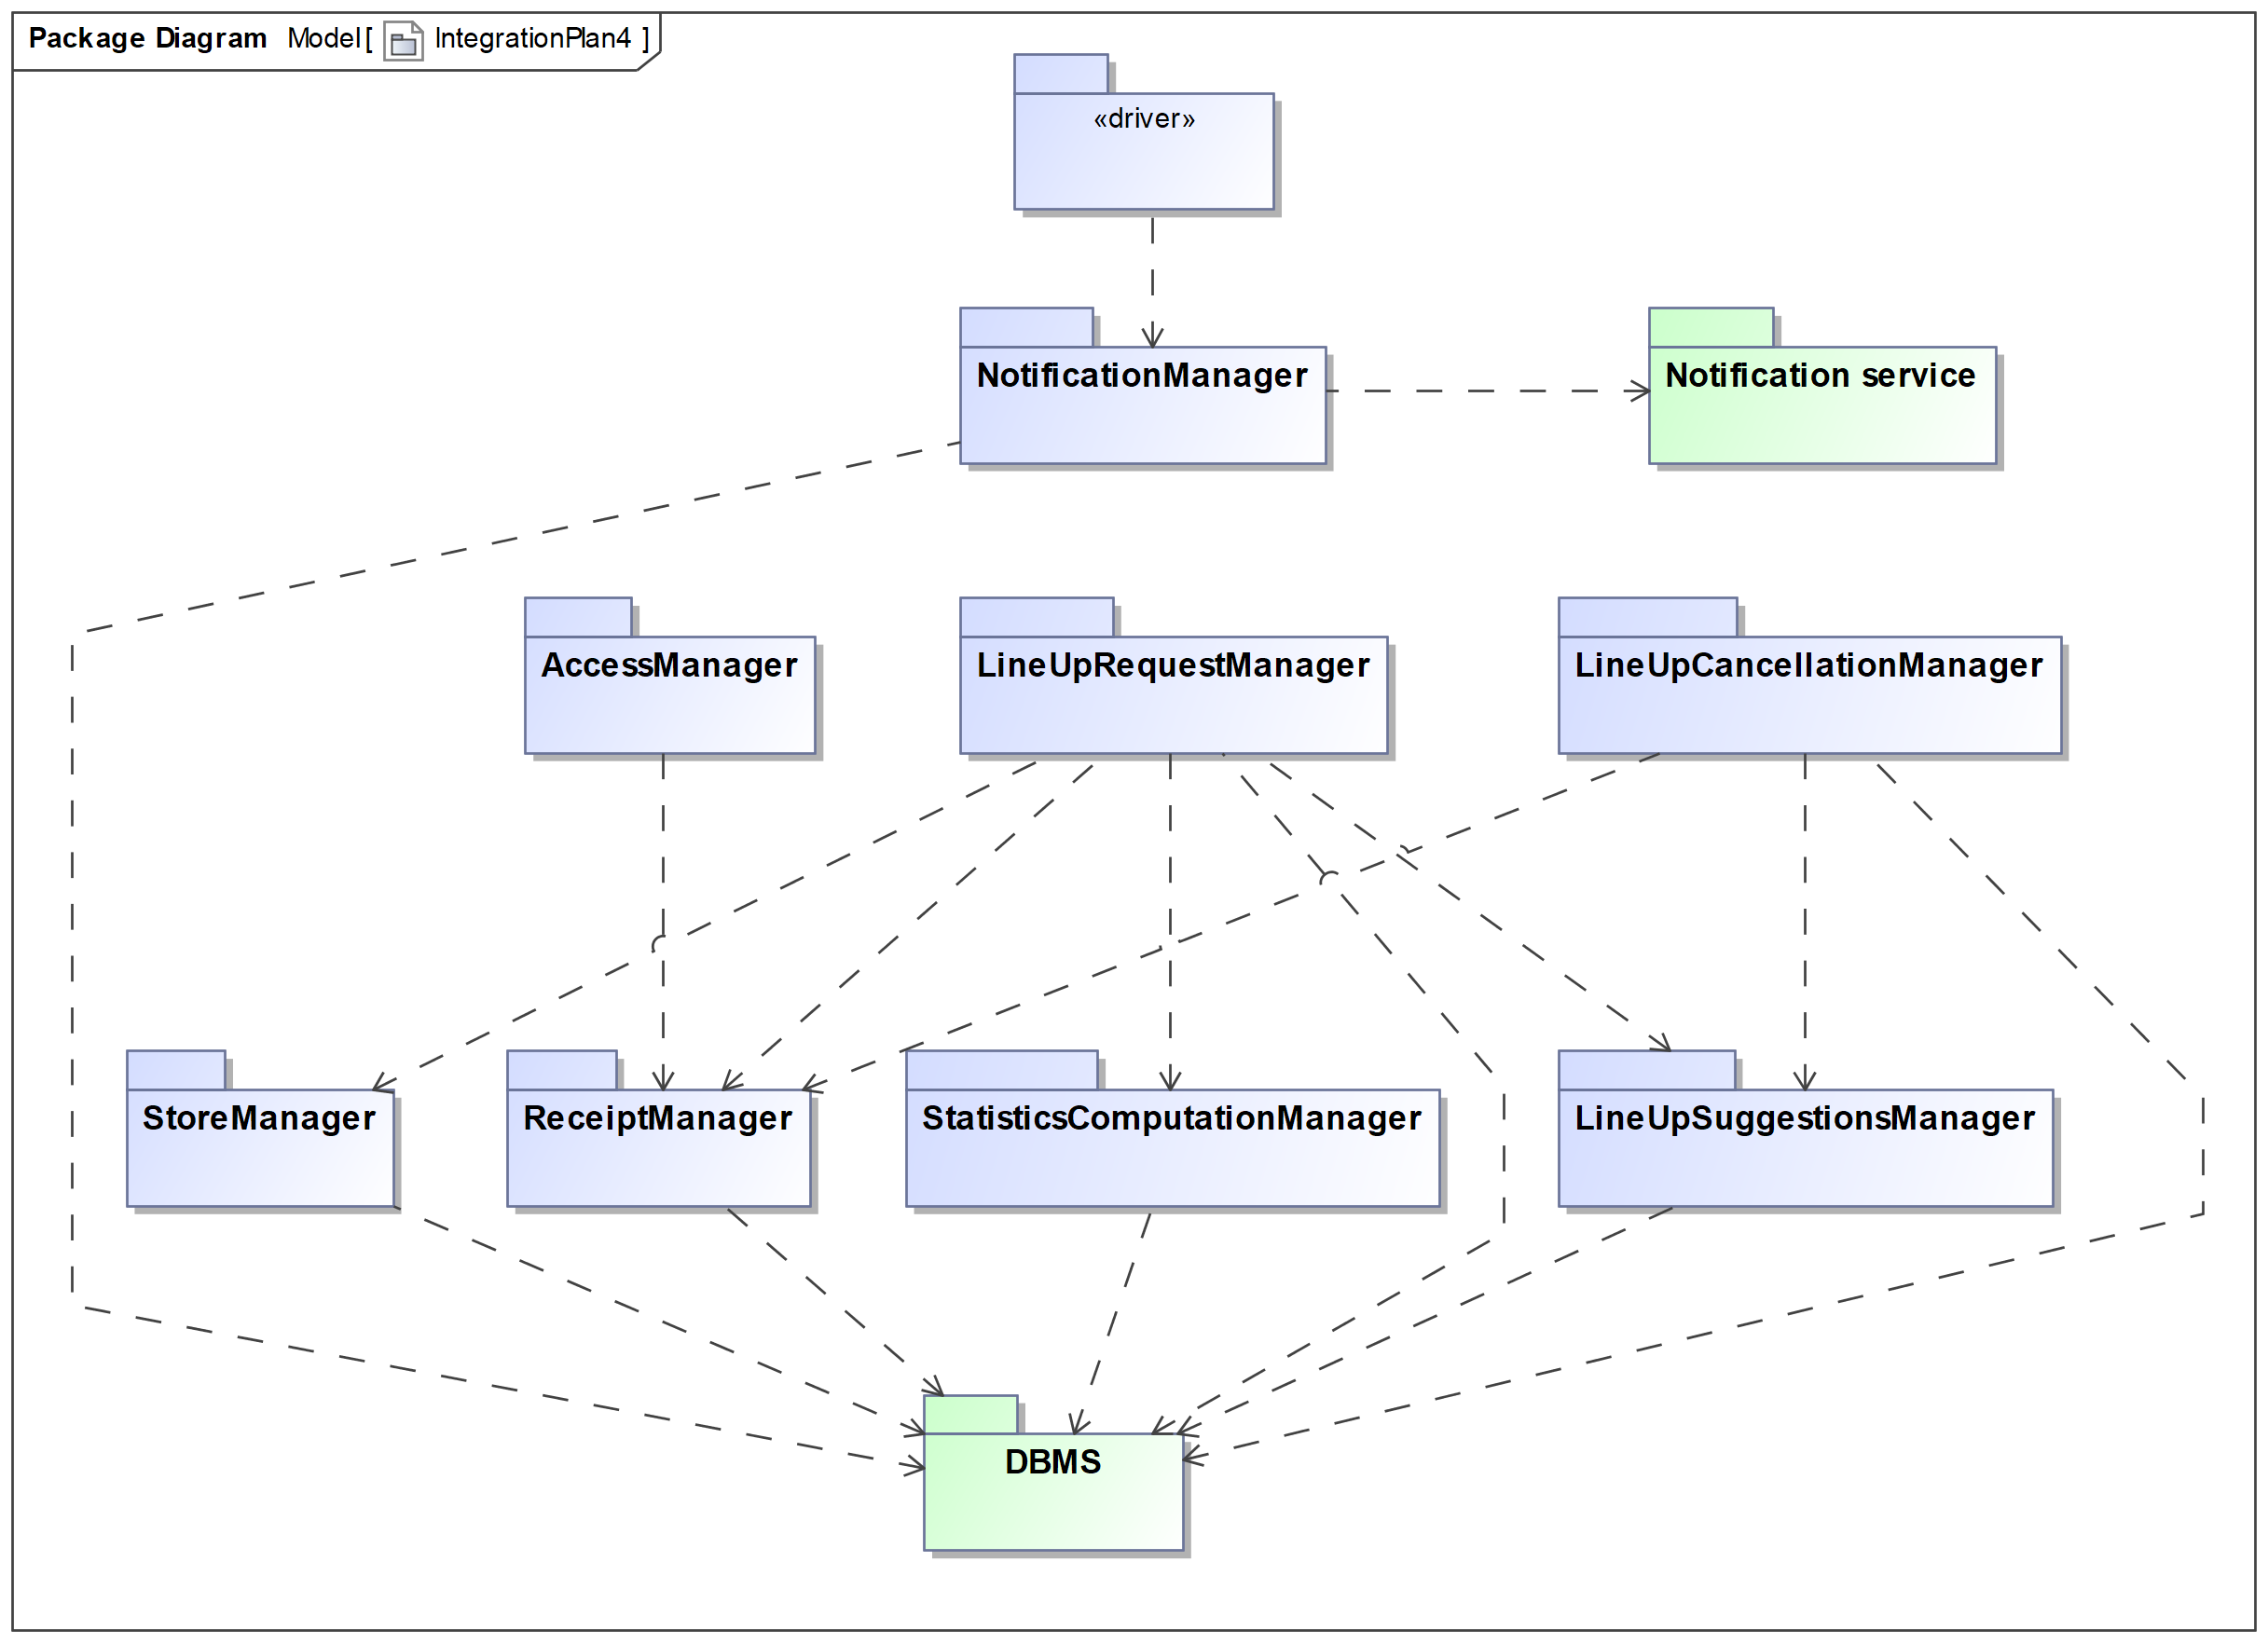
\includegraphics[width=15cm]{package__IntegrationPlan4.png}
	\end{figure}

	\end{minipage}

	\noindent\begin{minipage}{0.9\textwidth}
		
	\item Later, the implementation of AuthenticationManager and its integration with the Identity Provider can begin. 

	\begin{figure}[H]
    \centering
    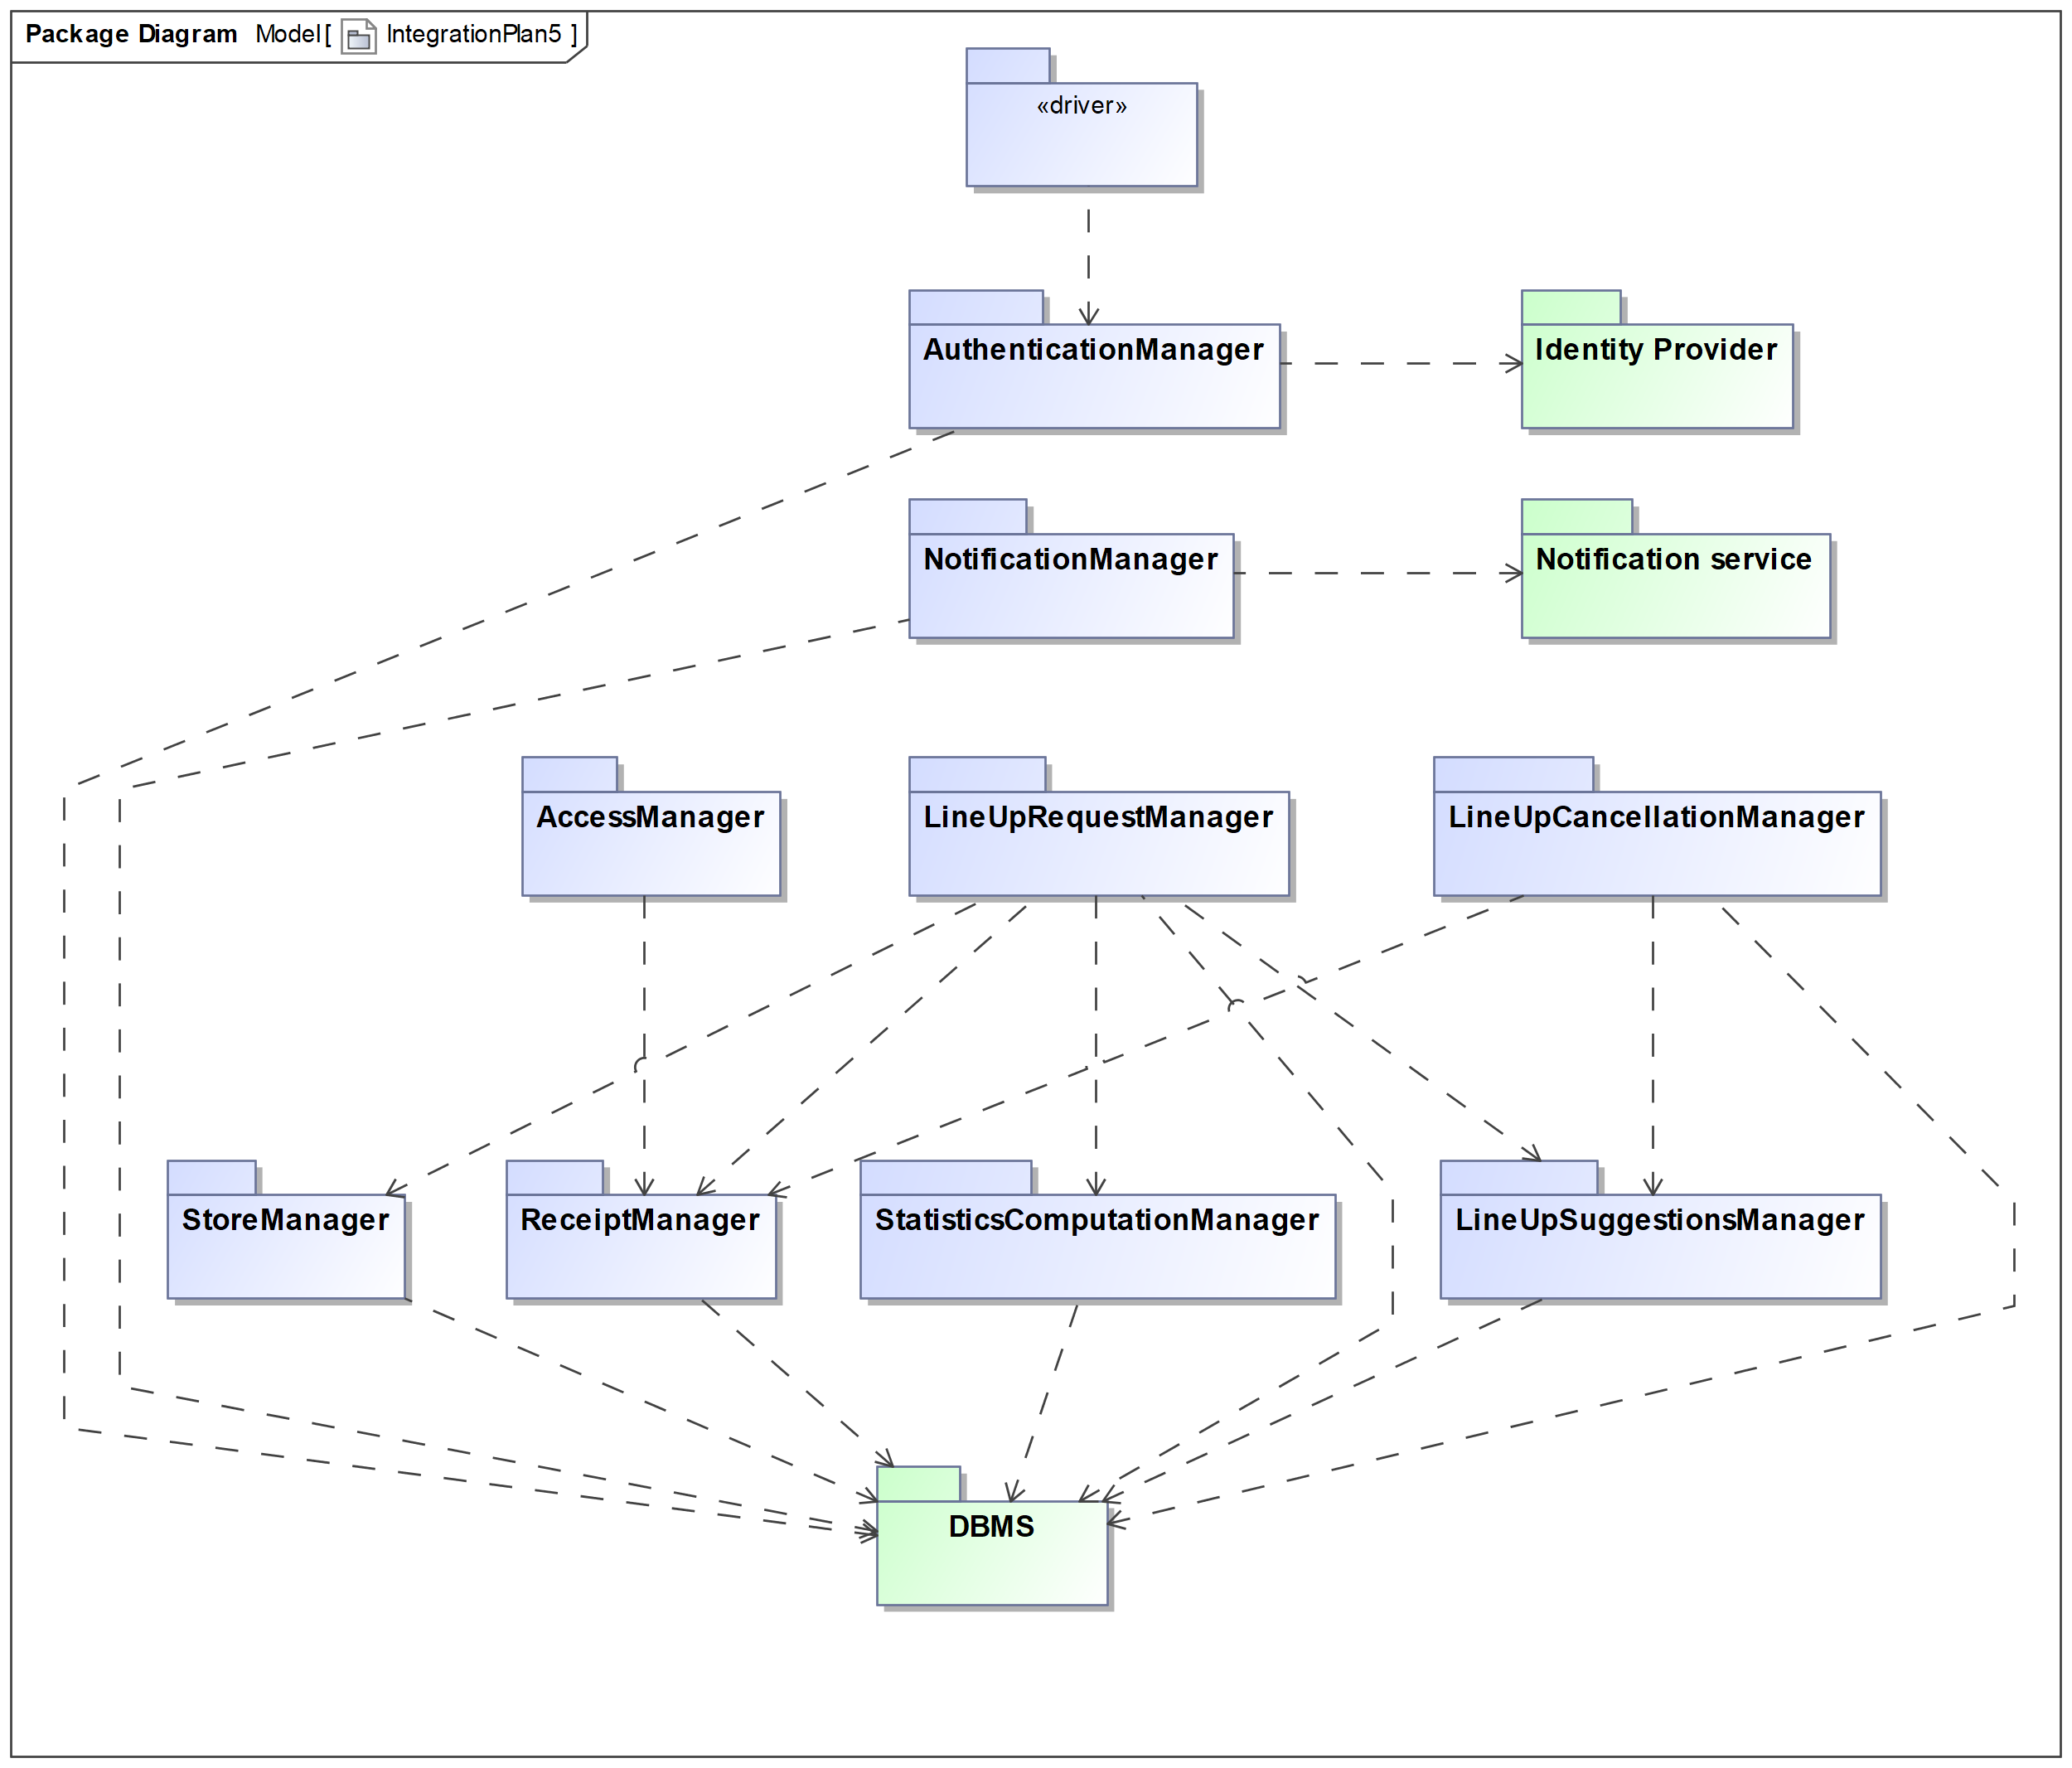
\includegraphics[width=15cm]{package__IntegrationPlan5.png}
	\end{figure}

	\end{minipage}

	\noindent\begin{minipage}{0.9\textwidth}
		
	\item Then, after the deployment of the Web Server component, its integration in the whole system is tested.

	\begin{figure}[H]
    \centering
    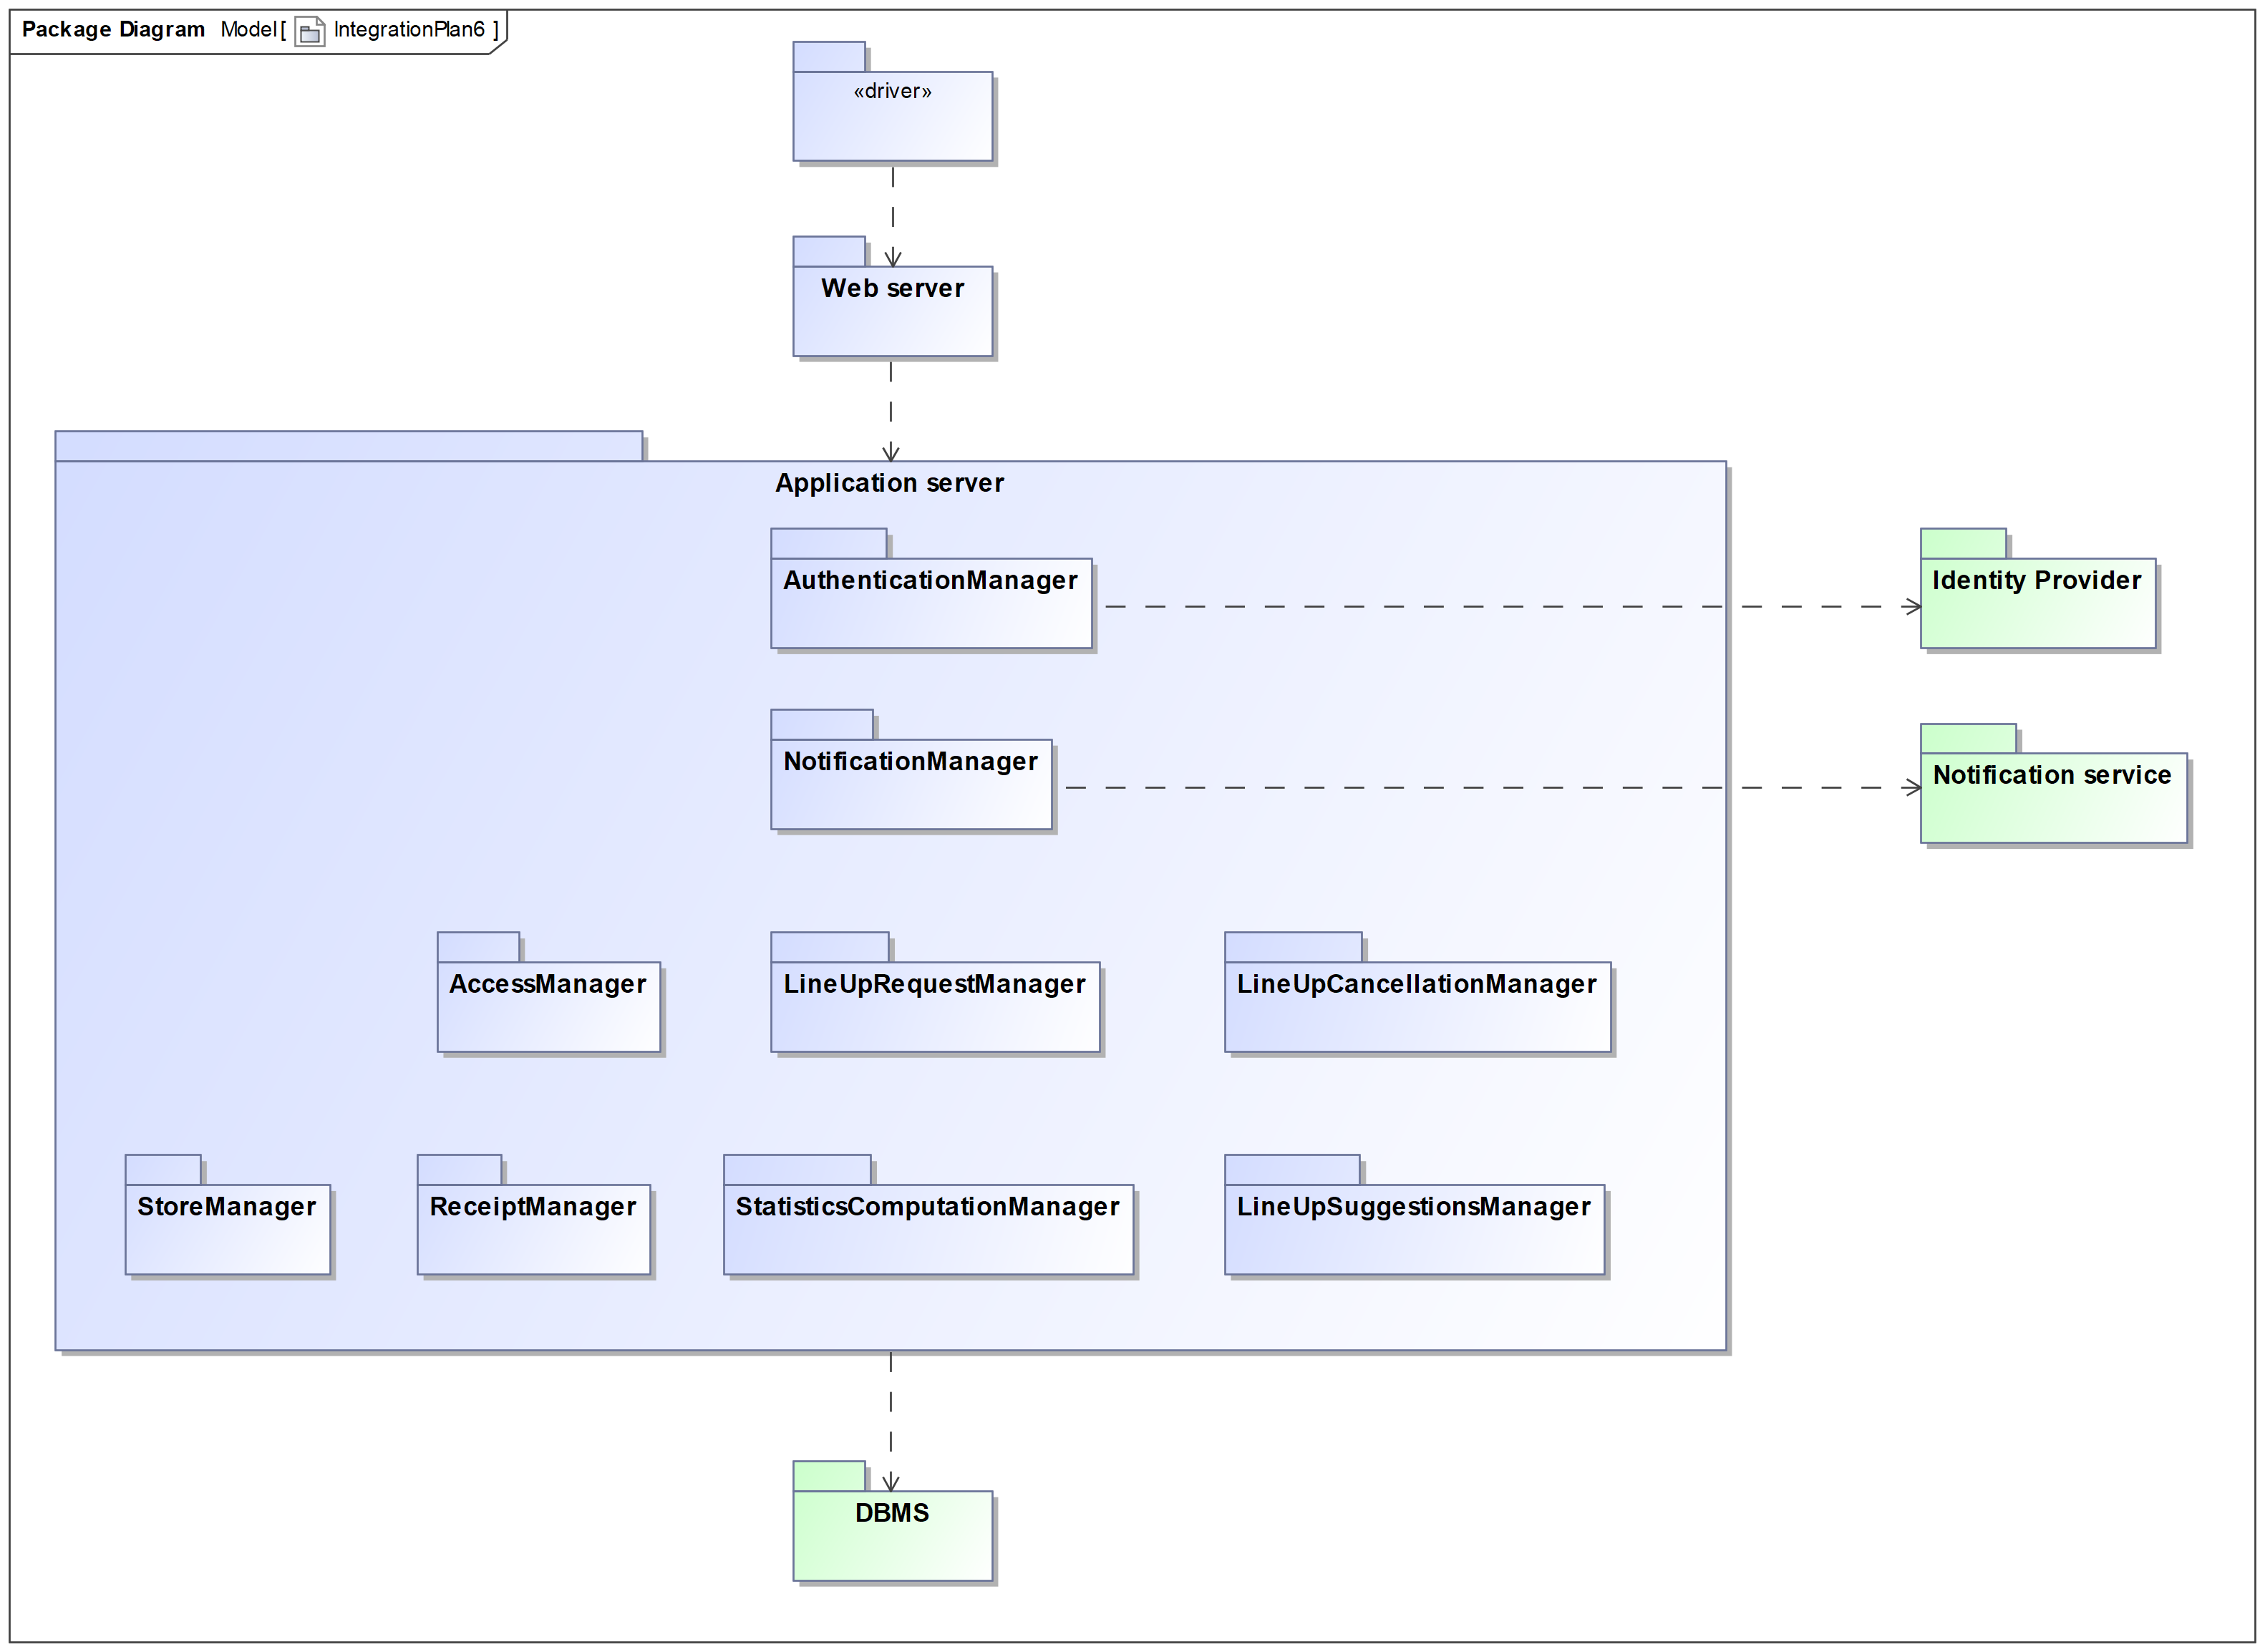
\includegraphics[width=\textwidth]{package__IntegrationPlan6.png}
	\end{figure}

	\end{minipage}

	\noindent\begin{minipage}{0.9\textwidth}
		
	\item Finally, the Phone Call Serice and the TripTimeEstimation Service are integrated into the system. IT devices, telephones, and receipt scanners are used to interact with the completed system.

	\begin{figure}[H]
    \centering
    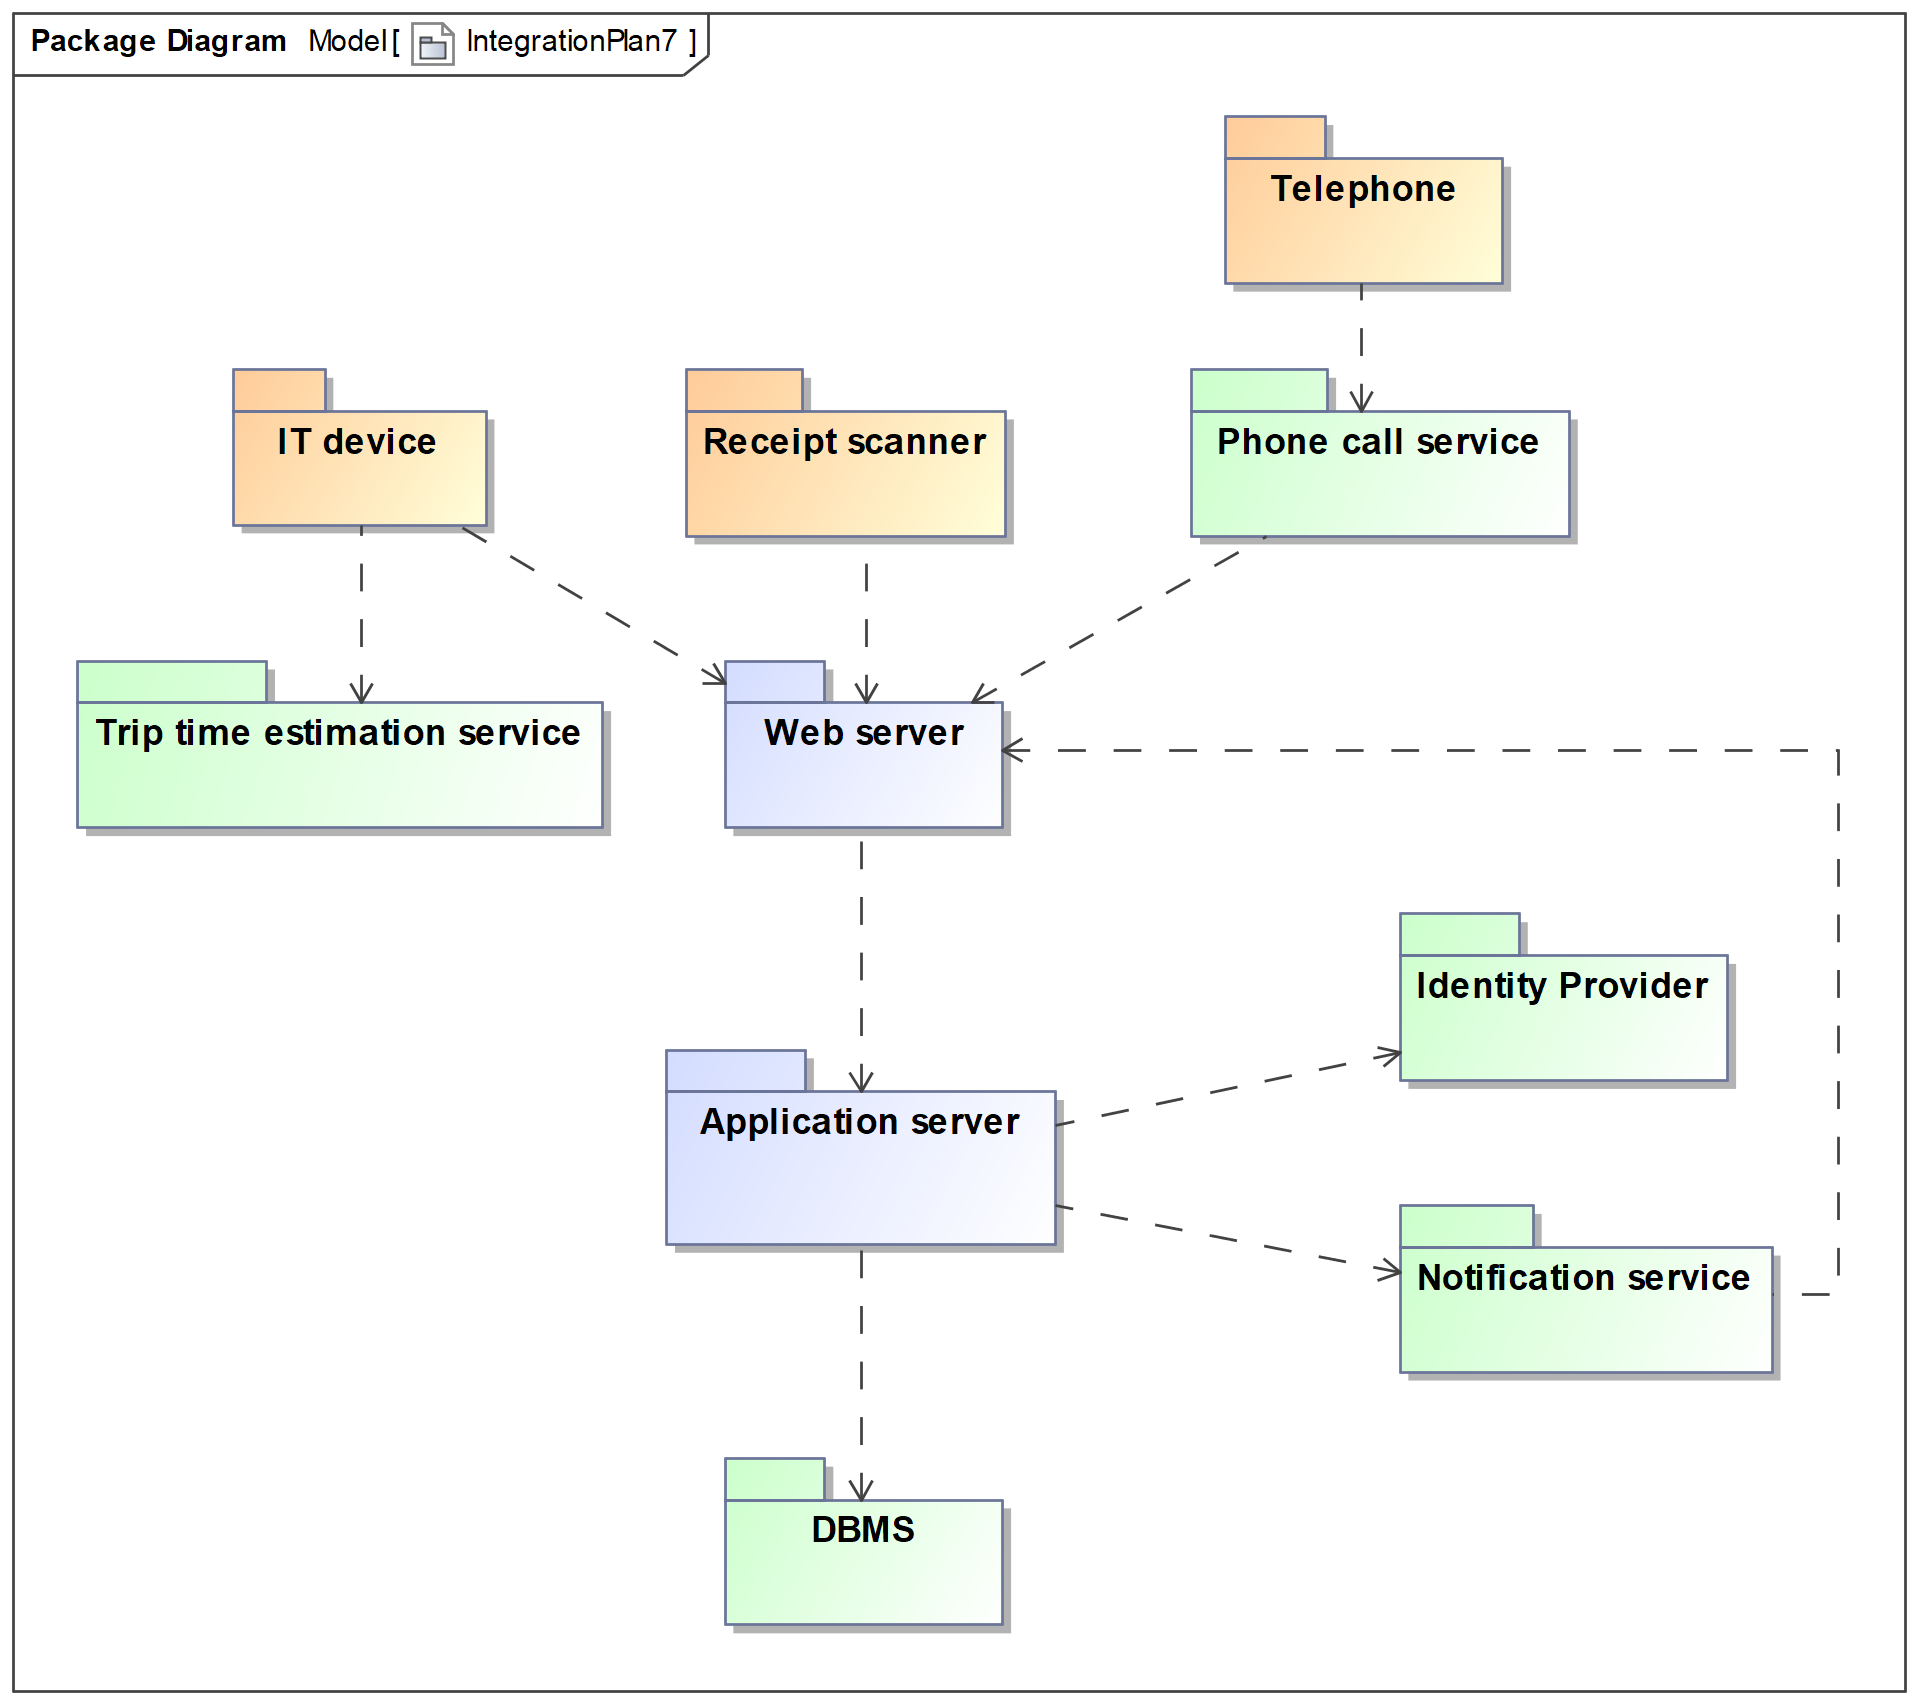
\includegraphics[width=12cm]{package__IntegrationPlan7.png}
	\end{figure}

	\end{minipage}

\end{enumerate}

\end{document}
%Testing plan
%* Implementation -> subsystem test (using driver) -> integrate -> integration test (for children)
%- DBMS integration testing
%- StoreManager
%- ReceiptManager
%- AccessManager
%- StatisticsComputationManager
%- LineUpSuggestionsManager
%- LineUpRequestManager
%- LineUpCancellationManager
%- notification servuce integration testing + NotificationManager
%- identity provider integration testing + AuthenticationManager
%- Web server tested it device + TripTimeEstimationService
%
